\documentclass{sigchi}

% Use this command to override the default ACM copyright statement (e.g. for preprints). 
% Consult the conference website for the camera-ready copyright statement.


%% EXAMPLE BEGIN -- HOW TO OVERRIDE THE DEFAULT COPYRIGHT STRIP -- (July 22, 2013 - Paul Baumann)
\toappear{LIDET is located inside the Department of Computer Science of the Institute of Mathematics and Statistics, at the University of S\~ao Paulo\\
Rua do Mat\~ao, 1010, CEP 05508-090, S\~ao Paulo, SP, Brazil\\
Telephone: +55 11 3091--9600\\

Daros is a MSc student, Vieira and Pereira are PhD students, and Corr\^ea da Silva is their advisor.\\

This manuscript was submitted in November 21st 2014 to the iGAM4ER 2014 competition (http://igam4er.org/) taking place in Paris, France, in December 13th and 14th 2014.
}
%% EXAMPLE END -- HOW TO OVERRIDE THE DEFAULT COPYRIGHT STRIP -- (July 22, 2013 - Paul Baumann)


% Arabic page numbers for submission. 
% Remove this line to eliminate page numbers for the camera ready copy
% \pagenumbering{arabic}


% Load basic packages
\usepackage{balance}  % to better equalize the last page
\usepackage{graphics} % for EPS, load graphicx instead
\usepackage{times}    % comment if you want LaTeX's default font
\usepackage{url}      % llt: nicely formatted URLs
\usepackage{tabu}
\usepackage{subcaption}
\usepackage{enumitem}
\usepackage{multicol}

% llt: Define a global style for URLs, rather that the default one
\makeatletter
\def\url@leostyle{%
  \@ifundefined{selectfont}{\def\UrlFont{\sf}}{\def\UrlFont{\small\bf\ttfamily}}}
\makeatother
\urlstyle{leo}


% To make various LaTeX processors do the right thing with page size.
\def\pprw{8.5in}
\def\pprh{11in}
\special{papersize=\pprw,\pprh}
\setlength{\paperwidth}{\pprw}
\setlength{\paperheight}{\pprh}
\setlength{\pdfpagewidth}{\pprw}
\setlength{\pdfpageheight}{\pprh}

% Make sure hyperref comes last of your loaded packages, 
% to give it a fighting chance of not being over-written, 
% since its job is to redefine many LaTeX commands.
\usepackage[pdftex]{hyperref}
\hypersetup{
bookmarksnumbered,
pdfstartview={FitH},
colorlinks,
citecolor=black,
filecolor=black,
linkcolor=black,
urlcolor=black,
breaklinks=true,
}

% create a shortcut to typeset table headings
\newcommand\tabhead[1]{\small\textbf{#1}}

% path of images
\graphicspath{{./images/}}

% Shared affiliations
\def\sharedaffiliation{%
\end{tabular}
\begin{tabular}{c}}

% To keep the url in the same font of the institution address
\newcommand{\urlwofont}[1]{\urlstyle{same}\url{#1}}

% Column types for text
\newcolumntype{L}[1]{>{\raggedright\let\newline\\\arraybackslash\hspace{0pt}}m{#1}}
\newcolumntype{C}[1]{>{\centering\let\newline\\\arraybackslash\hspace{0pt}}m{#1}}
\newcolumntype{R}[1]{>{\raggedleft\let\newline\\\arraybackslash\hspace{0pt}}m{#1}}

\newcommand{\refsectitle}[1]{\ref{#1}~(\nameref{#1})}

% End of preamble. Here it comes the document.
\begin{document}

% Define the name of the game
\newcommand{\gamename}{Sweet Switches}
\title{\gamename: a Digital Game to Foster Learning Computer Programming Skills}

\numberofauthors{4}
\author{
	\alignauthor Vin\'icius Kiwi Daros\\
		\email{vkdaros@ime.usp.br}
%
	\alignauthor Luiz Carlos Vieira\\
		\email{lvieira@ime.usp.br}
%
	\alignauthor Adalberto Bosco C. Pereira\\
		\email{bosco@ime.usp.br}
%
	\alignauthor Fl\'avio S. Corr\^ea da Silva\\
		\email{fcs@ime.usp.br}
%
	\sharedaffiliation  
		\affaddr{Laboratory of Interactivity and Digital Entertainment Technology (LIDET)}\\
		\affaddr{\urlwofont{http://www.ime.usp.br/~lidet}}
}
\maketitle

\begin{abstract}
Yada yada yada
\end{abstract}

\keywords{
	games; education; computer programming; logical thinking; Brazilian fauna
}

\category{K.3.1.}{Computer Uses in Education}{Computer-assisted instruction (CAI)}
\category{K.8.0.}{Personal Computing}{Games}

\section{Introduction}

	\renewcommand{\gamename}{\textit{\textbf{Sweet Switches}}}
	\newcommand{\gamenamept}{\textit{\textbf{Sabores Seletos}}}
	
	In all developed countries, primary school children have at least one class a week when they use a computer \cite{Istrate2010}, but so far computers have been mostly employed to aid in other disciplines and as a productivity tool. So that it has been argued that young people should be educated not only in the application and use of technology, but also in \textit{how it works} and what are its \textit{fundamental principles}. A report prepared for the UK Computing Research Committee \cite{Jones2009} particularly mentions the fact that UK students are now becoming disenchanted with the computer aided learning because they arrive at school with a much richer background in ICT (Information and Communication Technology). The report also advocates that if on one hand learning how to use computers can be seen as similar to learning how to read, on the other hand learning how to program computers is similar to learning how to write. They are both skills that everyone should have, even though only a minority will become professionals (writers or computer programmers).
	
	Despite grounded arguments both in favor and against the use of computers by children \cite{Istrate2010,Setzer2001} and the relevance of the so called ``computer literacy'' or ``computational thinking'' trend \cite{Wing2006,Atwood2012}, the study of computer programming elements at primary and secondary school is increasingly being acknowledged as equally important as other disciplines such as math or science. The main reason is that the skills required for programming computers are definitely valuable for education, since they involve procedural thinking, problem solving through trial and error, creativity, thinking about thinking, and the analysis and exploration of data \cite{Kahn1999}.

	The experience the authors of this paper have had in teaching basic computer programming at the graduation course in Administration at the University of S\~ao Paulo corroborates that even when employing tools that the students are required to use in their daily routines and are accustomed with -- such as the Microsoft Office Excel\footnote{\url{http://office.microsoft.com/excel}} with the Visual Basic for Applications (VBA) programming language -- the task of learning how to use control structures in planning and solving problems by iterative execution is still perceived as a tedious activity even for older students.
	
	As consequence, the authors have been working on the development of a digital game called \gamename~(\gamenamept~in Portuguese), which has educational intentions mainly related to the development of skills necessary for programming computational tasks, \textit{but not directly involving coding}. The game mechanics is based on planning and building a production line that gets increasingly more complex as the player improves his or her understanding of how the control flow works. The next sections will describe existing similar playful environments and games that served as inspiration and details of the game under development.

\section{Similar Existing Products}

	\subsection{Playful Environments used for Teaching Programming}
		Playful environments employed to teach programming to children usually rely on motivating the creation of code from fun interactions with the real world or by allowing children to create their own content. One of the first examples of these environments is LabVIEW \cite{Erwin2000}, used to help programing the behaviors of robots made of modular sensors and motors in the LEGO Mindstorms\footnote{http://mindstorms.lego.com}. It is a visual interface in which programs are built by stringing basic subroutines together in a block diagram, which can then be further reused as a new routines in higher levels.
		
		Another very popular example of playful environment is MIT's Scratch\footnote{http://scratch.mit.edu/} \cite{Resnick2009}. It is also a visual tool composed of graphical blocks that children snap together to move images or play sounds. The format of these blocks are carefully designed so they intuitively indicate syntax restrictions. For instance, a decision block (the ``if'' yellow block at figure~\ref{fig:scratch}) is C-shaped to suggest that other blocks can fit inside it.

	\subsection{Games used for Teaching Programming}
		There are also games used for teaching programming, but instead of allowing a free test-bed environment they are games that involve computer programming in the mechanics. One famous example is CodeCombat \cite{Saines2013}. This is an adventure game in which players control the hero character indirectly by programing behaviors through coding small functional actions such as move right, left, down and up, find nearest enemy and attack enemy. The game allows coding in many different programming languages, and includes important concepts like use of variables and repetition blocks.
	
		A very recent example is BBC's Doctor Who and and the Dalek \cite{BBC2014}. This is a platform game in which the player directly controls a Dalek cyborg \footnote{http://en.wikipedia.org/wiki/Dalek}, an extraterrestrial race from the British science fiction series \textit{Doctor Who}. The programming is used in the fantasy of the game as a manner of improving the cyborg abilities at the end of completed levels, like programming its jump or attack behaviors (as illustrated in figure~\ref{fig:dr-who}).

		\begin{figure}
			\centering
			\begin{subfigure}[!h]{0.5\columnwidth}
				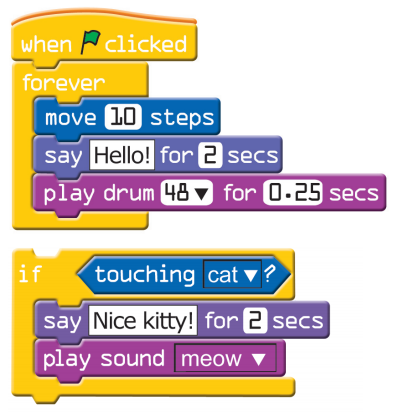
\includegraphics[width=\textwidth]{scratch}
				\caption{Sample programs from Scratch}
				\label{fig:scratch}
			\end{subfigure}%

			\begin{subfigure}[!h]{0.7\columnwidth}
				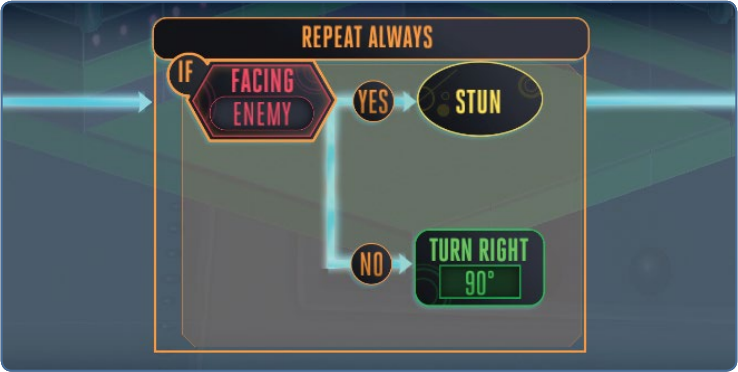
\includegraphics[width=\textwidth]{dr-who}
				\caption{Repetition block from a program in Dr. Who and the Dalek}
				\label{fig:dr-who}
			\end{subfigure}
			\caption{Programming in playful environments and games}
			\label{fig:samples}
		\end{figure}

	\subsection{Games involving Logistics}
		There are many games involving logistics, that is the management of the flow of resources between points to meet some requirements. 

\section{The Construction of \gamename}

	Scratch's site audience is between the ages of 8 and 16 (peaking at 12), with also a sizable group of adult participants \cite{Resnick2009}.
	
	Without control flow structures such as ``IF'' commands in programming languages, it is simply not possible to construct a program that is useful because the resolution of problems depends on \textit{making decisions} in some scope.
	
	A problem with the existing approaches using entertainment to motivate learning programming skills is that they are too focused on direct input of code.
	\begin{quotation}
		\noindent
		\textit{The ``everyone should learn to code'' movement [...] assumes that coding is the goal. Software developers tend to be software addicts who think their job is to write code. But it's not. Their job is to solve problems.} \cite{Atwood2012}
	\end{quotation}
	
	The mechanics behind this puzzle is indeed very simple. And this is intentional. The game is doomed to become boring, as the player understands well enough on how to manage the flow of ice cream production and the game fantasy no longer brings novelty and curiosity.
	
\section{Educational Aspects Addressed}

\section{Concept Art}

	Here are some sketches of the concept art planned for \gamename.
	\begin{center}
		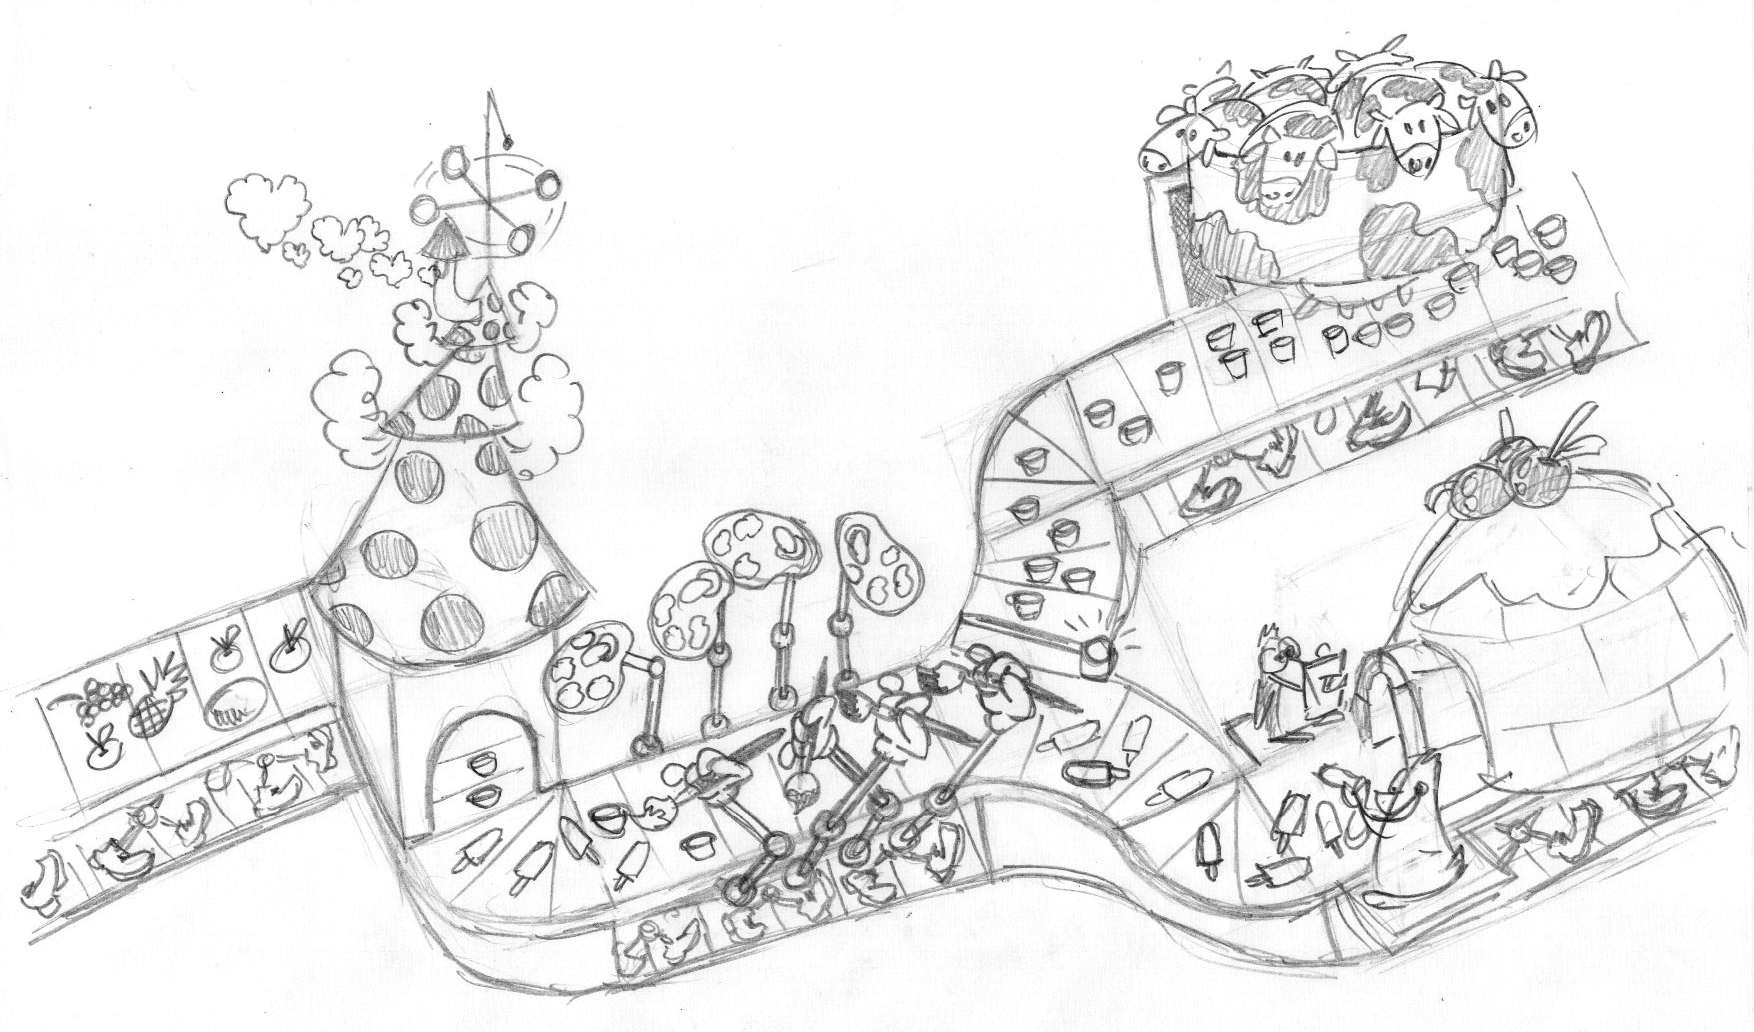
\includegraphics[width=0.9\columnwidth]{01}
		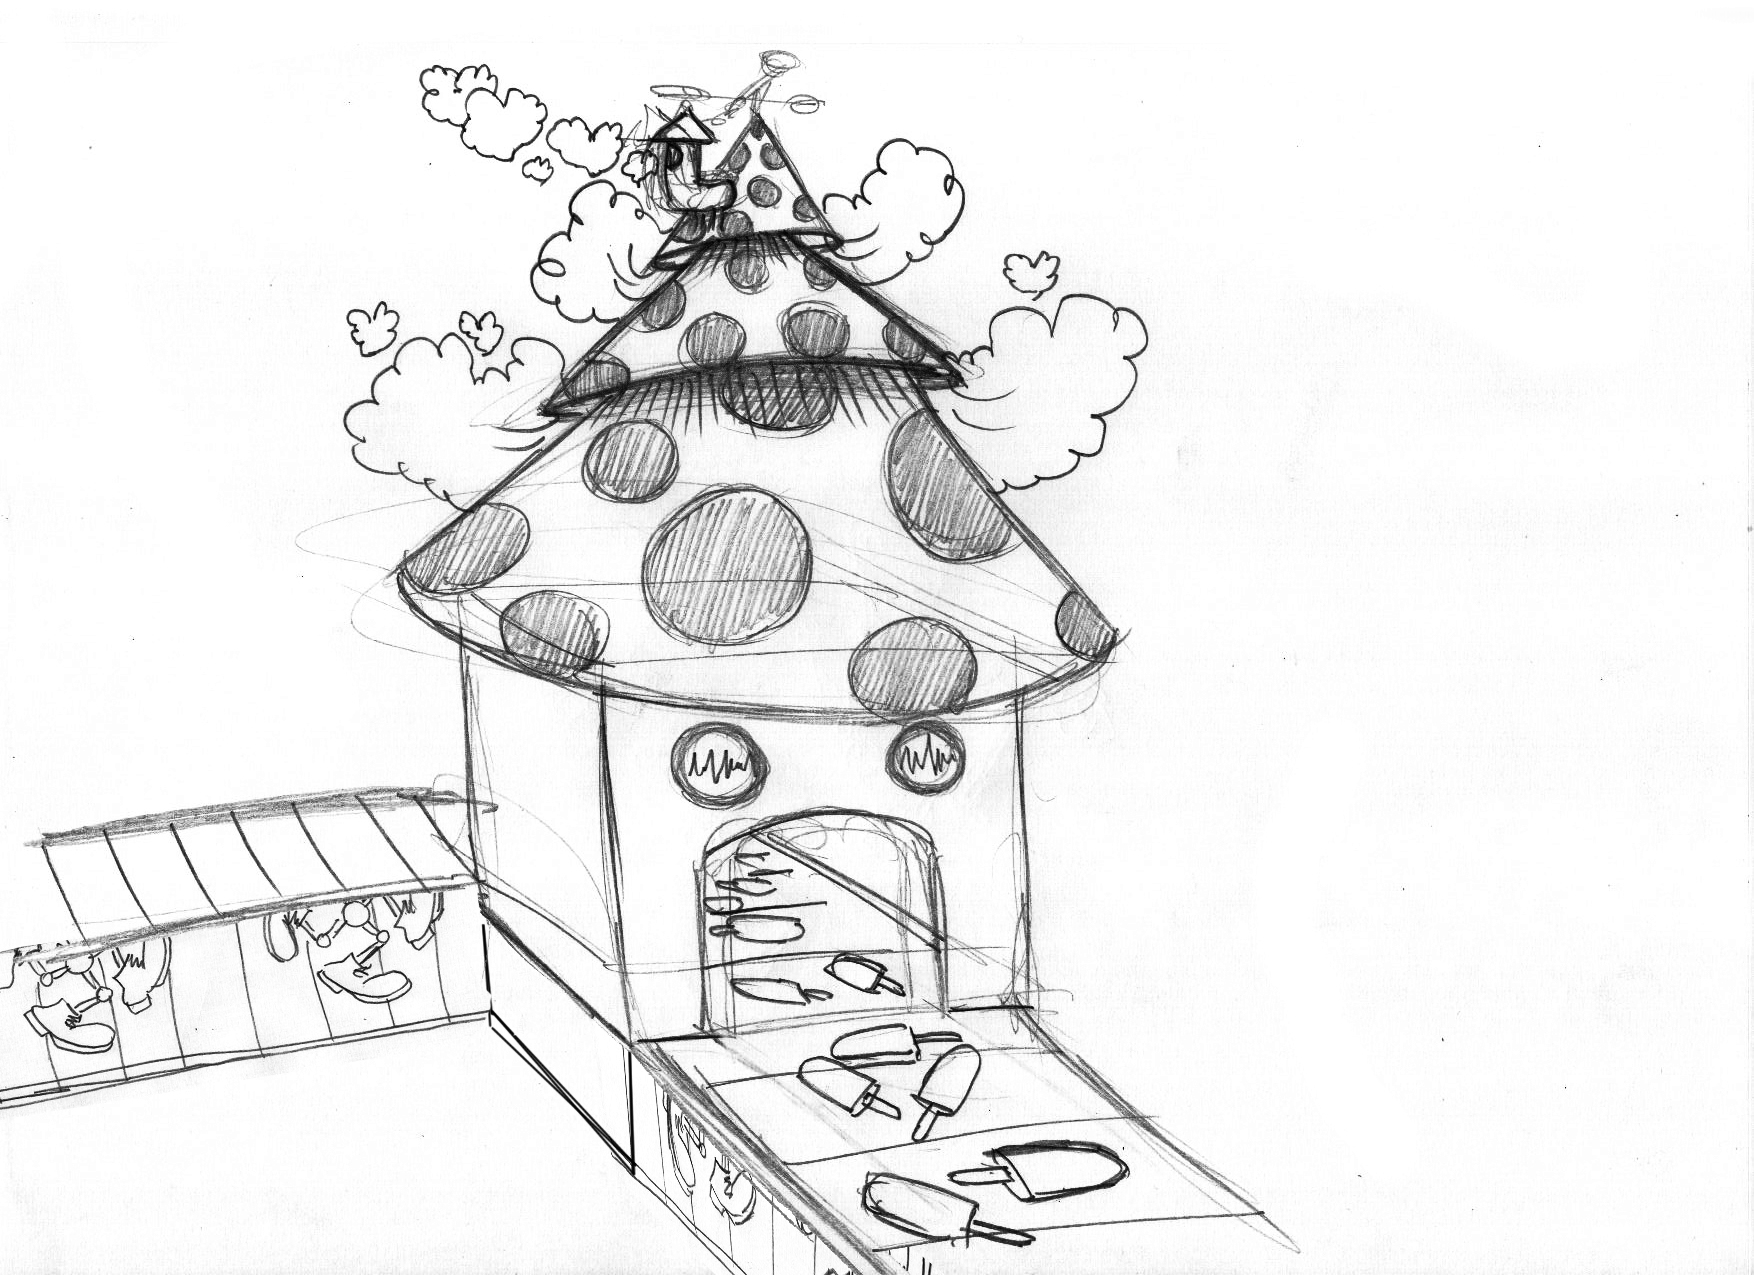
\includegraphics[width=0.9\columnwidth]{02}
		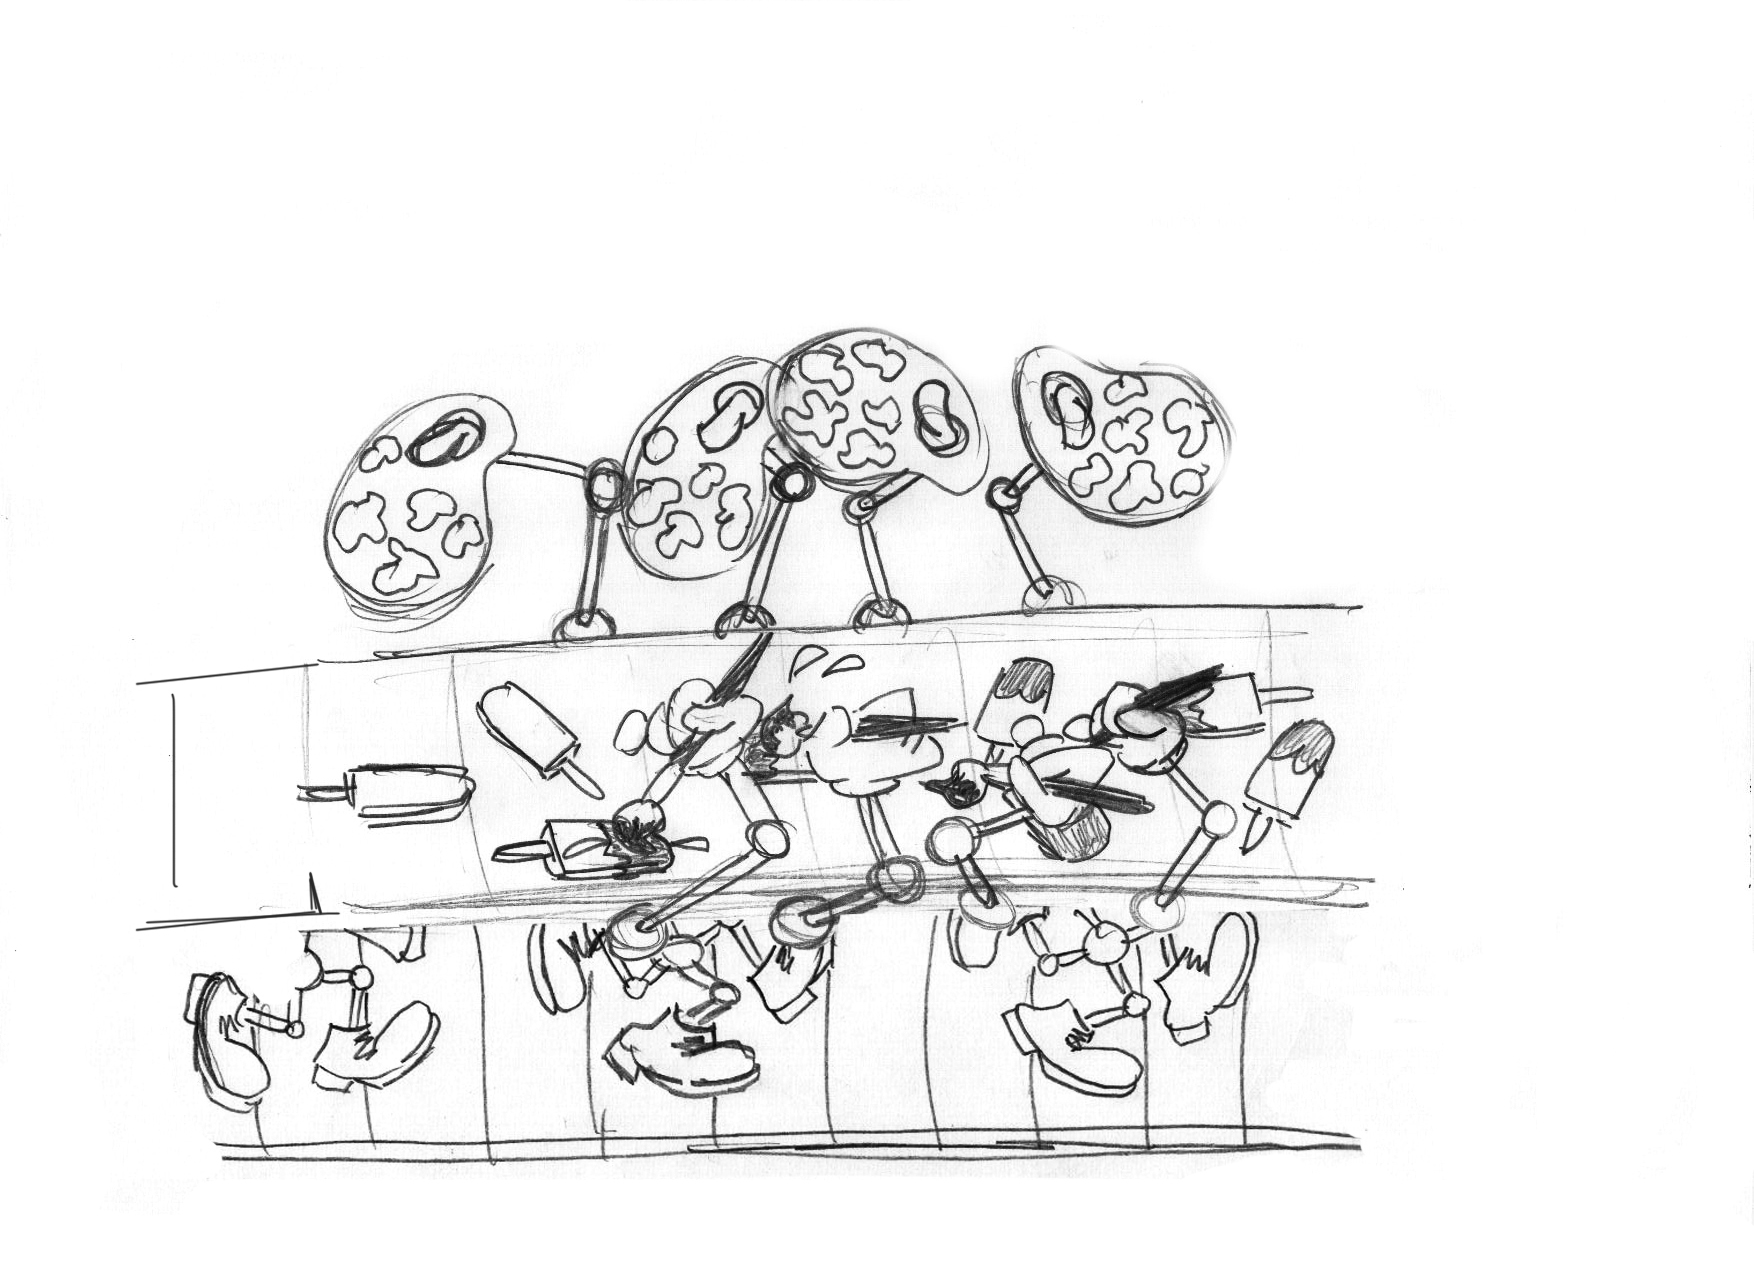
\includegraphics[width=0.9\columnwidth]{03}
		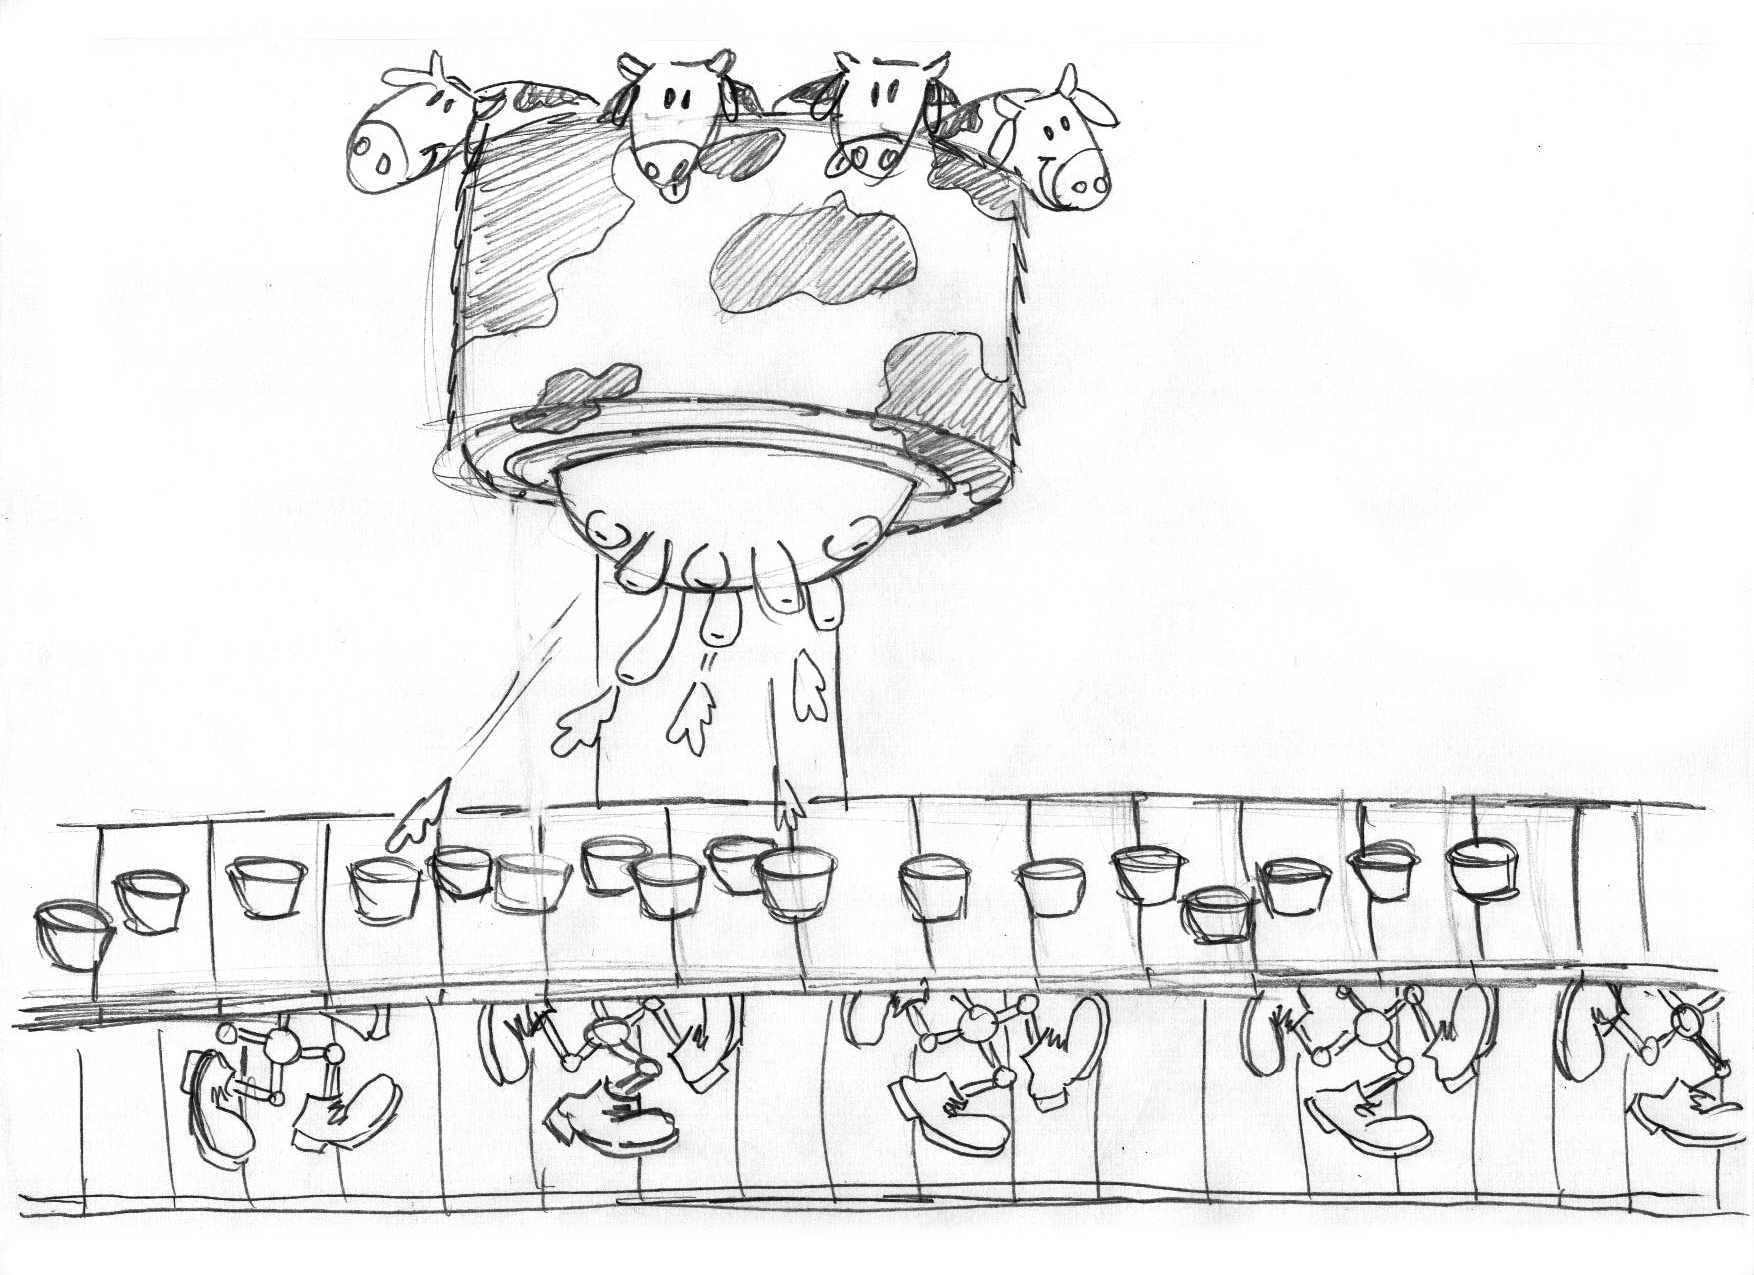
\includegraphics[width=0.9\columnwidth]{04}
		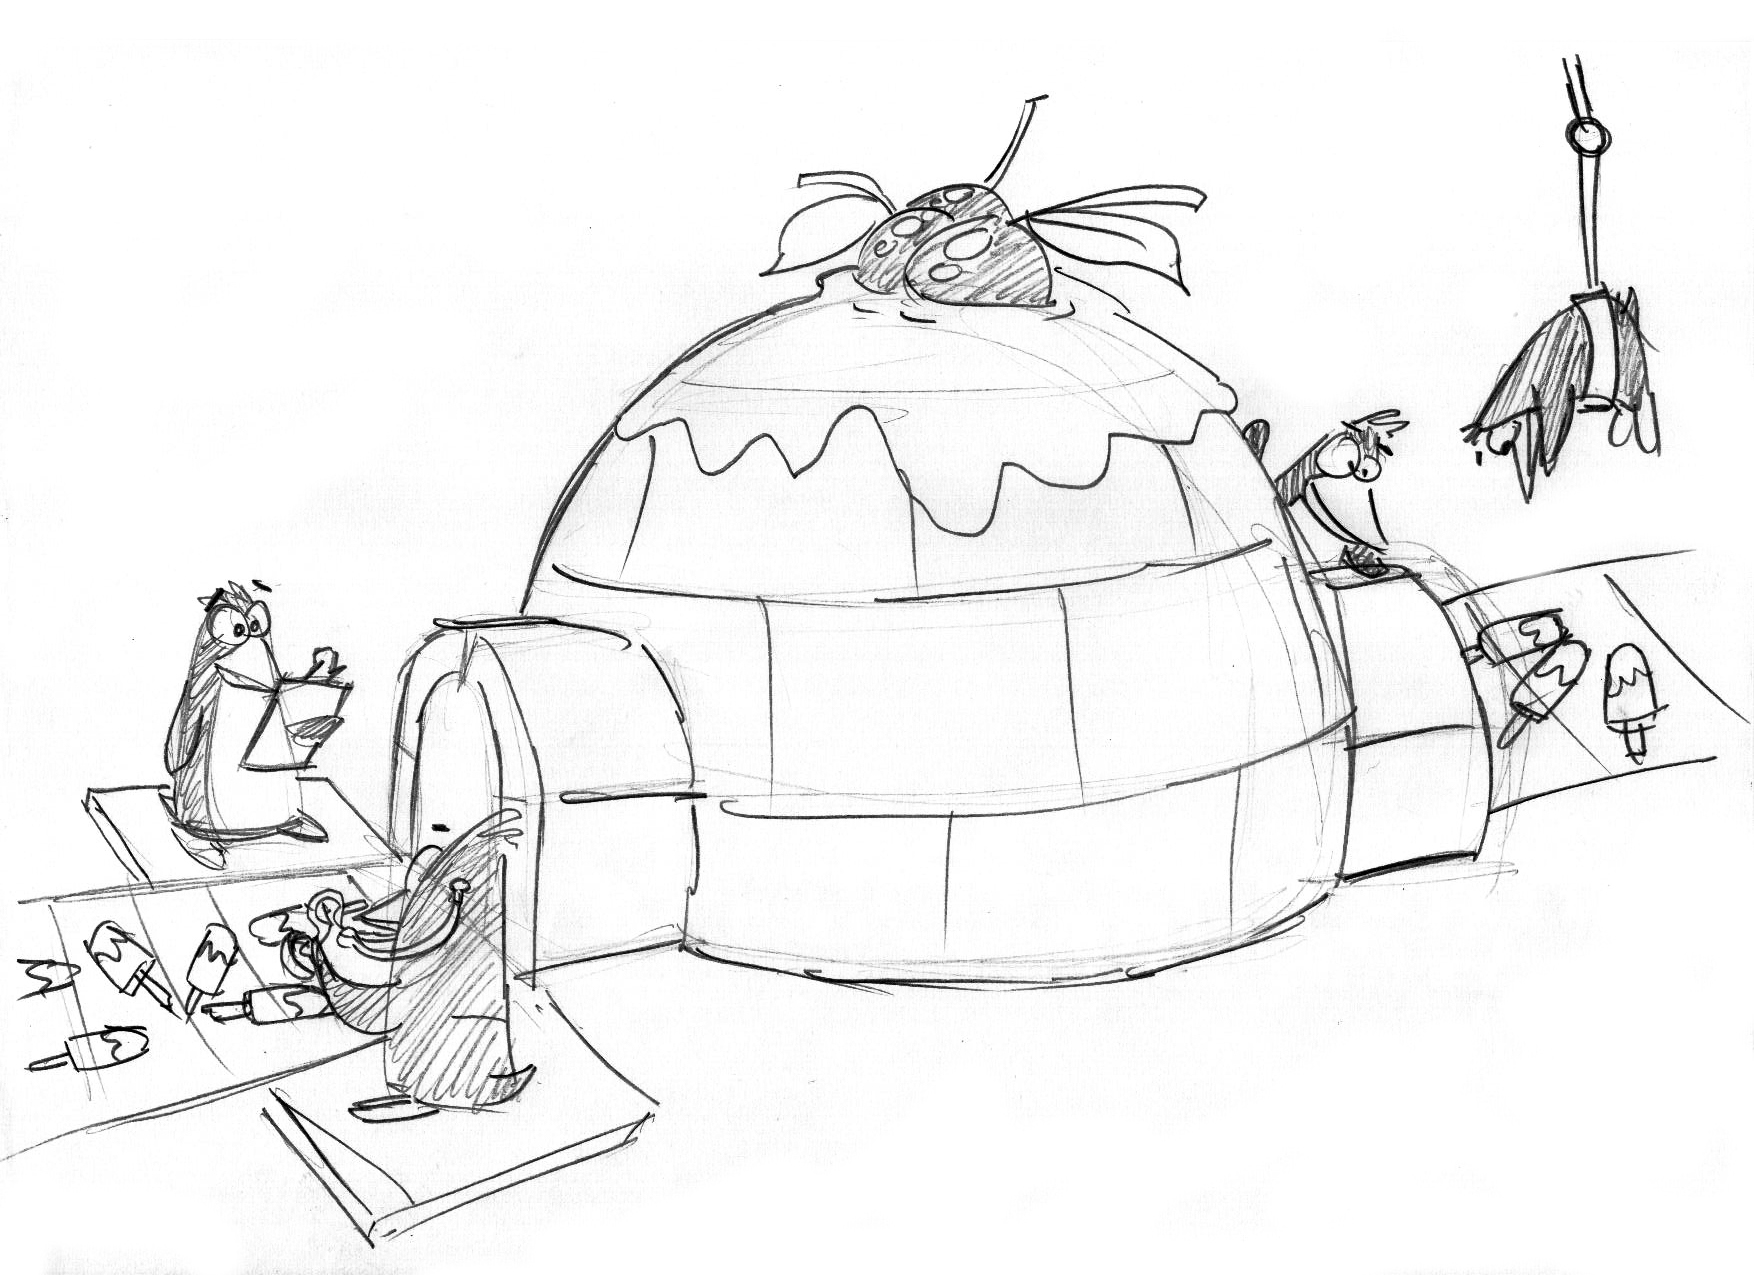
\includegraphics[width=0.9\columnwidth]{05}
		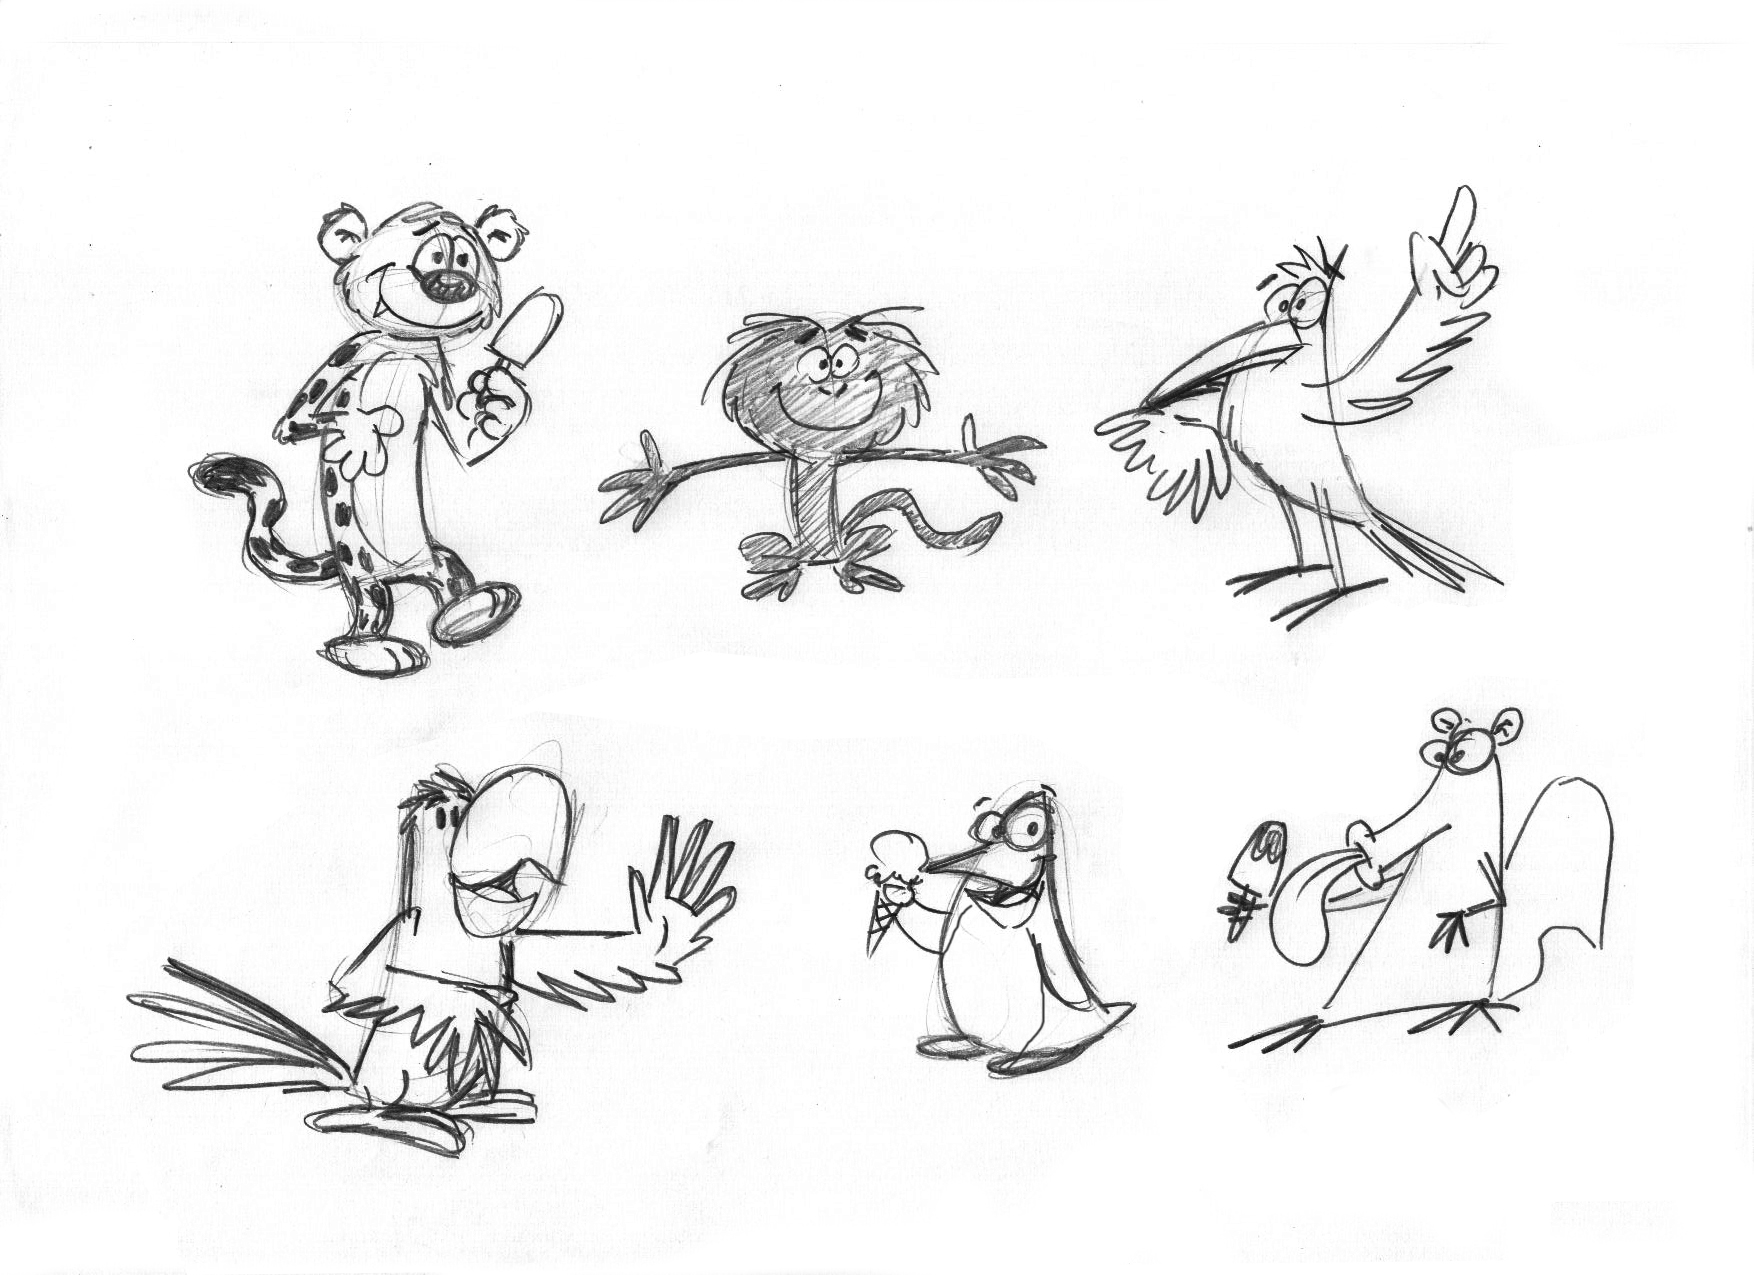
\includegraphics[width=0.9\columnwidth]{06}
	\end{center}

\section{Acknowledgments}

	The authors would like to thank CAPES (\textit{Coordena\c{c}\~ao de Aperfei\c{c}oamento de Pessoal de N\'ivel Superior}) and CRI (Center for Research and Interdisciplinarity) for the financial support, and the artists Danilo Gabriel Rios and Salvador Oliva Junior for the concept art.

% Balancing columns in a ref list is a bit of a pain because you
% either use a hack like flushend or balance, or manually insert
% a column break.  http://www.tex.ac.uk/cgi-bin/texfaq2html?label=balance
% multicols doesn't work because we're already in two-column mode,
% and flushend isn't awesome, so I choose balance.  See this
% for more info: http://cs.brown.edu/system/software/latex/doc/balance.pdf
%
% Note that in a perfect world balance wants to be in the first
% column of the last page.
%
% If balance doesn't work for you, you can remove that and
% hard-code a column break into the bbl file right before you
% submit:
%
% http://stackoverflow.com/questions/2149854/how-to-manually-equalize-columns-
% in-an-ieee-paper-if-using-bibtex
%
% Or, just remove \balance and give up on balancing the last page.
%
\balance

\bibliographystyle{acm-sigchi}
\bibliography{igamer_bib}
\end{document}
